\clearpage% Flush earlier floats (otherwise order might not be correct)
\newpage


\section{Results}\label{sec:results}
This section presents a painting placement solution to the painting placement instances described in table~\ref{tab:instances}.
Hyperparameter values used to obtain results in this section are in table~\ref{tab:hyperparameters-values}.
Statistics for each instance are in table~\ref{tab:statistics}.

Hyperparameter values in table~\ref{tab:hyperparameters-values} are set to their recommended values
from hyperparameter testing in section~\ref{sec:hyper-parameters}.
The hyperparameter not set to the recommended values is \verb|maxNumberOfIter|.
It is set to 500 instead of a value from the recommended range \numrange{100}{150}.
The reason is to possibly find a better painting placement solution in exchange for more computation time.

The recommendation to remove orientation penalization by setting \verb|orientationWeights| to $\langle 1,1,1\rangle$ is followed.
As described in hyperparameter testing, it should produce a population with a better on-average objective and a faster-decreasing trend in objective value.
Also, the population size is set to 75 times the instance size.
It is the midpoint of the recommended interval \numrange{50}{100}.
Lastly, population division is set to the same values in listing~\ref{lst:computation-submission-dataset}.
It means keeping an elitism strategy and injecting random individuals into the reproductive plan.


\begin{table}[h!]
    \caption{Hyperparameter values used to obtain results}
    \label{tab:hyperparameters-values}
    \begin{threeparttable}
        \begin{tabular}{ll}
            \hline
            \textbf{Hyperparameter}                           & \textbf{Value}                                         \\ \hline
            \verb|maxNumberOfIter|                            & 500                                                    \\ \hline
            \verb|populationSize|                             & 75 times the instance size                             \\ \hline
            \verb|maximumWildCardCount|                       & 1                                                      \\ \hline
            \verb|orientationWeights|                         & $\langle 1,1,1 \rangle$                                \\ \hline
            \verb|populationDivisionCounts|                   & elitism, random                                        \\ \hline
            \verb|initialPopulationDivisionCounts|            & 0.7 random, 0.3 greedy                                 \\ \hline
            \verb|overlappingPenalizationConstant|            & \begin{tabular}[c]{@{}l@{}}
                                                                    4 times the diagonal length\\ of the layout
            \end{tabular} \\ \hline
            \verb|outsideOfAllocatedAreaPenalizationConstant| & 0                                                      \\ \hline
        \end{tabular}
        \begin{tablenotes}
            \small
            \item Hyperparameter description is in table~\ref{tab:hyperparameters-description}.
        \end{tablenotes}
    \end{threeparttable}
\end{table}

\begin{table}[h!]
    \caption{Statistics of the last iteration}
    \label{tab:statistics}
    \begin{threeparttable}
        \begin{tabular}{lllll}
            \hline
            \textbf{Instance name} &
            \textbf{\begin{tabular}[c]{@{}l@{}}
                        Best obj.\\ value
            \end{tabular}} &
            \textbf{\begin{tabular}[c]{@{}l@{}}
                        Worst obj.\\ value
            \end{tabular}} &
            \textbf{\begin{tabular}[c]{@{}l@{}}
                        Obj.\\ mean
            \end{tabular}} &
            \textbf{\begin{tabular}[c]{@{}l@{}}
                        Standard\\ deviation
            \end{tabular}}                    \\ \hline
            random\_10                    & 1136.11  & 3438.01 & 1640.91 & 460.76 \\ \hline
            random\_20                   & 5417.8  & 11629.59  & 7209.22 & 1400.13  \\ \hline
            packing\_10                   & 669.48 & 2369.11 & 1142.96 & 383.22 \\ \hline
            packing\_20                 & 6219.13 & 12283.41 & 8140.29 & 1450.09 \\ \hline
            cluster\_3\_6                 & 3921.68 & 11121.96 & 6317.36  & 1844.99 \\ \hline
            cluster\_4\_5 & 4887.04    & 12088.99     & 7177.9    & 1767.67    \\ \hline
            biased\_sparse\_cluster\_3\_5         & TODO & TODO & TODO  & TODO \\ \hline
            london\_gallery\_wall         & 2759.65 & 15764.31 & 5440.9  & 2633.81 \\ \hline
        \end{tabular}
        \begin{tablenotes}
            \small
            \item Instance description is in table~\ref{tab:instances}.
        \end{tablenotes}
    \end{threeparttable}
\end{table}

\begin{figure}[h!]
    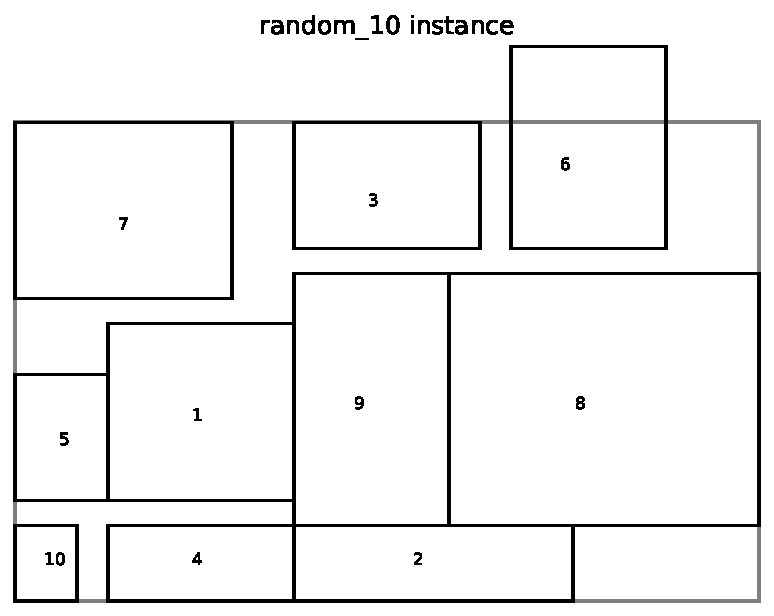
\includegraphics[width=0.8\textwidth, center]{visualizations/visualization_random_10}
    \caption[Painting placement solution for the random\_10 instance]
        {Painting placement solution for the random\_10 instance.
    There is one overlapping pair for paintings 6 and 9.}
    \label{fig:results:visualization-random-10}
\end{figure}

\begin{figure}[h!]
    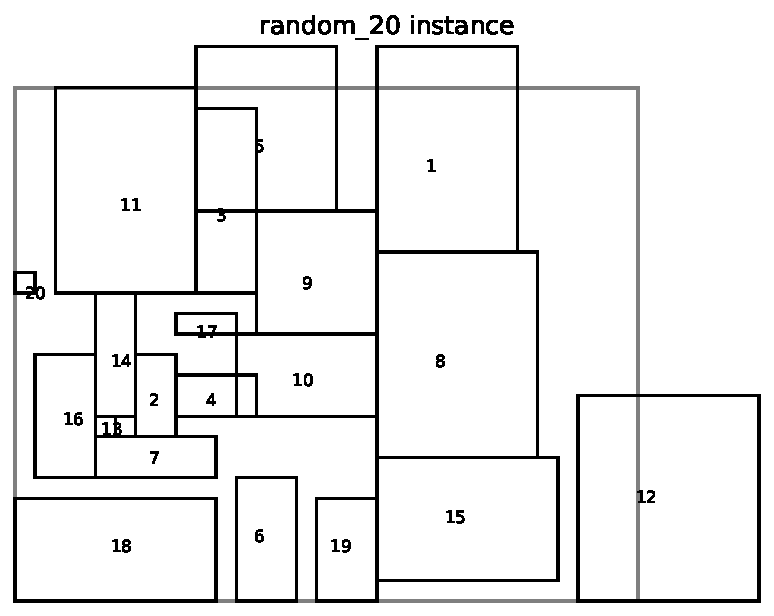
\includegraphics[width=0.8\textwidth, center]{visualizations/visualization_random_20}
    \caption[Painting placement solution for the random\_20 instance]
        {Painting placement solution for the random\_20 instance.
    There are two overlapping pairs, 3–5 and 4–10.}
    \label{fig:results:visualization-random-20}
\end{figure}

\begin{figure}[h!]
    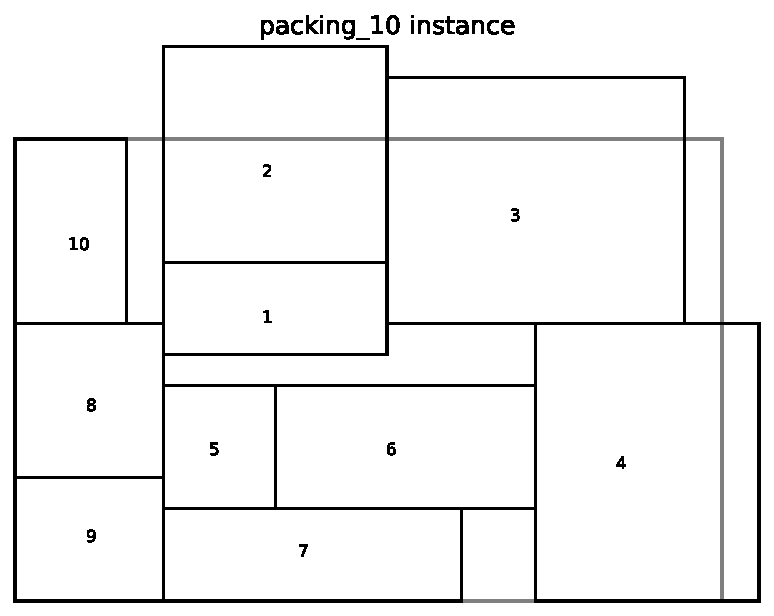
\includegraphics[width=0.8\textwidth, center]{visualizations/visualization_packing_10}
    \caption[Painting placement solution for the packing\_10 instance]
        {Painting placement solution for the packing\_10 instance.
    There are no overlappings.}
    \label{fig:results:visualization-packing-10}
\end{figure}

\begin{figure}[h!]
    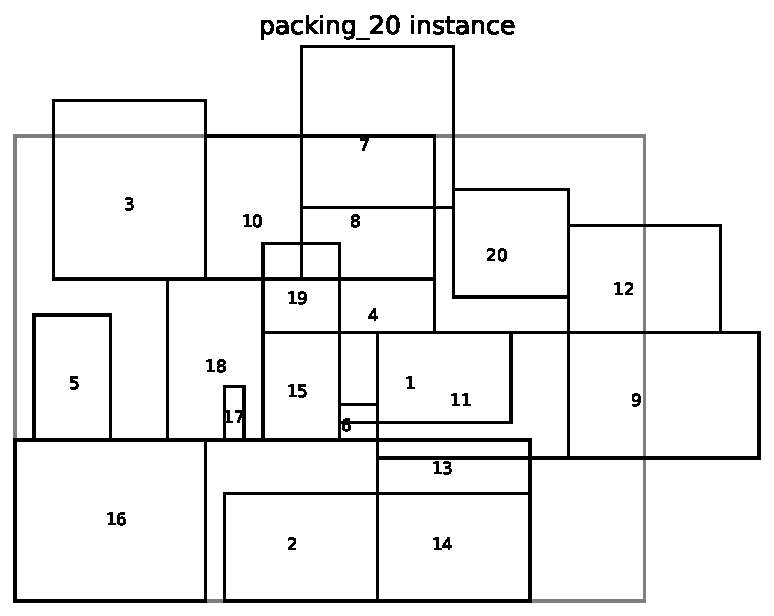
\includegraphics[width=0.8\textwidth, center]{visualizations/visualization_packing_20}
    \caption[Painting placement solution for the packing\_20 instance]
        {Painting placement solution for the packing\_20 instance.
    There are eight overlappings.}
    \label{fig:results:visualization-packing-20}
\end{figure}

\begin{figure}[h!]
    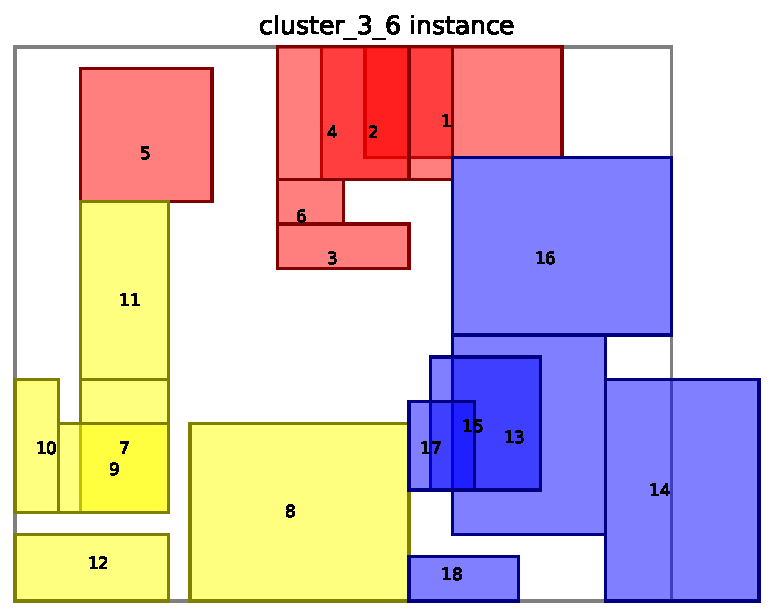
\includegraphics[width=0.8\textwidth, center]{visualizations/visualization_cluster_3_6}
    \caption[Painting placement solution for the cluster\_3\_6 instance]
        { Painting placement solution for the cluster\_3\_6 instance.
    Three groups of paintings, \numrange{1}{6}, \numrange{7}{12}, and \numrange{13}{18}, are marked using different colors.
    There are 4 overlappings.}
    \label{fig:results:visualization-cluster-3-6}
\end{figure}

\begin{figure}[h!]
    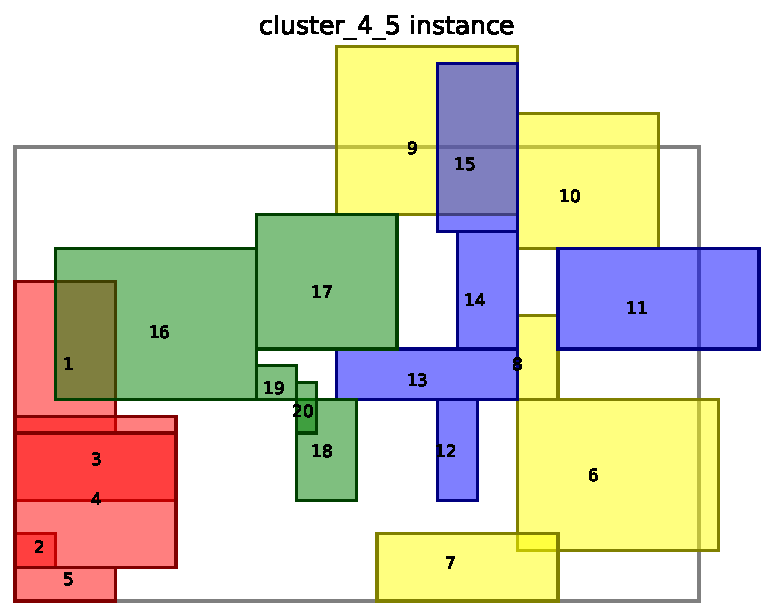
\includegraphics[width=0.8\textwidth, center]{visualizations/visualization_cluster_4_5}
    \caption[Painting placement solution for the cluster\_4\_5 instance]
        { Painting placement solution for the cluster\_4\_5 instance.
    Four groups of paintings, \numrange{1}{5}, \numrange{6}{10}, \numrange{11}{15}, and \numrange{15}{20}, are marked using different colors.
    There are 8 overlappings.}
    \label{fig:results:visualization-cluster-4-5}
\end{figure}

\begin{figure}[h!]
%    \includegraphics[width=0.8\textwidth, center]{visualizations/visualization_biased_sparse_cluster}
    
\includegraphics[width=0.8\textwidth, center]{placeholder}
    \caption
    {TODO biased sparse cluster}
    \label{fig:results:visualization-biased-sparse-cluster}
\end{figure}

\begin{figure}[h!]
    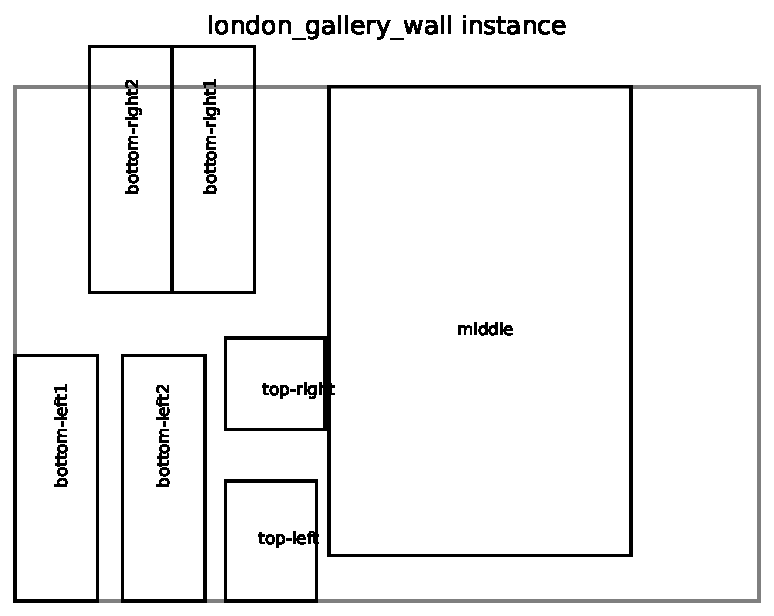
\includegraphics[width=0.8\textwidth, center]{visualizations/visualization_london_gallery_wall}
    \caption[Painting placement solution for the london\_gallery\_wall instance]
        { Painting placement solution for the london\_gallery\_wall instance.
    Paintings are marked using their original position in figure~\ref{fig:london-wall}.
    There are no overlappings.}
    \label{fig:results:visualization-london-gallery-wall}
\end{figure}


